\documentclass[conference]{IEEEtran}
\IEEEoverridecommandlockouts
% The preceding line is only needed to identify funding in the first footnote. If that is unneeded, please comment it out.
\usepackage{cite}
\usepackage{amsmath,amssymb,amsfonts}
\usepackage{algorithmic}
\usepackage{graphicx}
\usepackage{textcomp}
\usepackage{xcolor}
\usepackage{hyperref}
\usepackage{longtable}
\usepackage{tabularx}
\usepackage{tcolorbox}
\usepackage{array}
\usepackage{booktabs}
\tcbuselibrary{skins}

% Define styles for user and assistant boxes
\newtcolorbox{userbox}{colback=blue!5,colframe=blue!40!black,title=User}
\newtcolorbox{assistantbox}{colback=gray!10,colframe=black,title=Assistant}

\def\BibTeX{{\rm B\kern-.05em{\sc i\kern-.025em b}\kern-.08em
    T\kern-.1667em\lower.7ex\hbox{E}\kern-.125emX}}
\begin{document}

\title{HASHIRU: Hierarchical Agent System for Hybrid Intelligent Resource Utilization}

\author{\IEEEauthorblockN{Kunal Pai}
\IEEEauthorblockA{\textit{UC Davis} \\
kunpai@ucdavis.edu}
\and
\IEEEauthorblockN{Parth Shah}
\IEEEauthorblockA{\textit{Independent Researcher} \\
helloparthshah@gmail.com}
\and
\IEEEauthorblockN{Harshil Patel}
\IEEEauthorblockA{\textit{UC Davis} \\
hpppatel@ucdavis.edu}
\and
\IEEEauthorblockN{Saisha Shetty}
\IEEEauthorblockA{\textit{UC Davis} \\
spshetty@ucdavis.edu}
}

\maketitle

\section{Introduction}\label{sec:introduction}

Rapid advancements in Large Language Models (LLMs) are reshaping Artificial Intelligence (AI) with profound capabilities in language understanding, generation, reasoning, and planning \cite{brown2020language, devlin2019bert, raffel2020exploring}. This progress drives the development of autonomous AI agents, shifting focus from single to Multi-Agent Systems (MAS) where collaborative teams tackle complex problems beyond individual scope \cite{dorri2018multi, wooldridge2009introduction}. Collaborative MAS show significant potential in diverse domains like scientific discovery \cite{boiko2023emergent}, software engineering \cite{qian2023communicative}, data analysis, and strategic decision-making \cite{wang2023decision}. The increasing complexity of tasks, demonstrated by benchmarks requiring advanced mathematical reasoning (e.g., GSM8K \cite{cobbe2021gsm8k}, SVAMP \cite{patel2021svamp}), coding (e.g., HumanEval \cite{chen2021codex}, CoDocBench \cite{pai2024codocbench}), and graduate-level technical knowledge \cite{phan2025humanitysexam}, highlights the need for agentic systems to effectively coordinate diverse cognitive resources \cite{wen2024benchmarkingcomplexinstructionfollowingmultiple}.

Despite this potential, contemporary agentic frameworks face significant limitations. Many are \textbf{rigid}, relying on predefined roles and static structures hindering adaptation to dynamic tasks \cite{zhang2023building}. \textbf{Resource obliviousness} is common; systems often lack mechanisms to monitor and optimize computational resources like API costs, memory, and CPU load, leading to inefficiency, especially when scaling or deploying in resource-constrained environments \cite{park2023generative}. This is often worsened by reliance on powerful, costly proprietary cloud LLMs. \textbf{Model homogeneity}, defaulting to a single powerful LLM for all sub-tasks, misses efficiency gains from a diverse ecosystem including smaller, specialized, or local models \cite{zhou2023agents}. While \textbf{tool use} is fundamental \cite{yao2022react, parisi2022talm}, agents' ability to autonomously \textbf{create and integrate new tools} remains limited, restricting dynamic extension and self-improvement without human intervention \cite{wang2023voyager}.

To address these challenges, we introduce \textbf{HASHIRU (Hierarchical Agent System for Hybrid Intelligent Resource Utilization)}, a novel MAS framework enhancing flexibility, resource efficiency, and adaptability. HASHIRU employs a hierarchical structure led by a central ``CEO'' agent dynamically managing specialized ``employee'' agents instantiated on demand. A core tenet is its \textbf{hybrid intelligence} approach, strategically prioritizing smaller (e.g., 3B--7B), locally-run LLMs (often via Ollama \cite{ollama}) for cost-effectiveness and efficiency. While prioritizing local resources, the system flexibly integrates external APIs and potentially more powerful models when justified by task complexity and resource availability, under the CEO's management.

The primary contributions are:
\begin{enumerate}
    \item A novel MAS architecture combining \textbf{hierarchical control} with \textbf{dynamic, resource-aware agent lifecycle management} (hiring/firing). This management is governed by computational budget constraints (cost, memory, concurrency) and includes an economic model with hiring/firing costs to discourage excessive churn.
    \item A \textbf{hybrid intelligence model} prioritizing cost-effective, local LLMs while adaptively incorporating external APIs and larger models, optimizing the efficiency-capability trade-off.
    \item An integrated mechanism for \textbf{autonomous API tool creation}, allowing dynamic functional repertoire extension.
    \item An \textbf{economic model} (hiring/firing fees) for agent management, promoting efficient resource allocation and team stability.
\end{enumerate}

This paper details HASHIRU's design and rationale. Section \ref{sec:background} discusses related work in agent architectures, dynamic management, resource allocation, model heterogeneity, and tool use. Section 3 elaborates on the architecture and core mechanisms. Section 4 presents experimental results (or outlines planned experiments), followed by discussion and conclusion in Sections 5 and 6.

\section{Background and Related Work} \label{sec:background}

Intelligent agent concepts have evolved from early symbolic AI \cite{russell2010artificial, shoham1994agent} to LLM-dominated frameworks leveraging models for reasoning, planning, and interaction \cite{wang2023survey, xi2023rise}. HASHIRU builds on this, addressing current limitations.

\subsection{Agent Architectures: Hierarchy and Dynamics}
MAS architectures vary, including flat, federated, and hierarchical \cite{dorri2018multi, horling2004survey}. Hierarchical models offer clear control and task decomposition but risk bottlenecks and rigidity \cite{gaston2005agenta,gaston2005agentb}. HASHIRU uses a \textbf{CEO-Employee hierarchy} for centralized coordination but distinguishes itself through \textbf{dynamic team composition}. Unlike systems with static hierarchies or predefined roles (e.g., CrewAI \cite{crewai}, ChatDev \cite{qian2023communicative}), HASHIRU's CEO dynamically manages the employee pool based on runtime needs and resource constraints.

\subsection{Dynamic Agent Lifecycle Management}
Dynamic MAS composition is crucial for complex environments \cite{valckenaers2005trends}. Agent creation/deletion triggers often relate to task structure or environmental changes. HASHIRU introduces a specific mechanism where the CEO makes \textbf{hiring and firing decisions} based on a cost-benefit analysis considering agent performance, operational costs (API fees, inferred compute), memory footprint (tracked explicitly as a percentage of available resources), and concurrency limits. HASHIRU also incorporates an \textbf{economic model} with explicit ``starting bonus'' (hiring) and ``invocation'' (usage) costs. This economic friction aims to prevent excessive initialization or usage for marginal gains and promote team stability, a nuance often missing in simpler dynamic strategies.

\subsection{Resource Management and Agent Economies}
Resource awareness is critical for scalable MAS. Economic research explores mechanisms like market-based auctions or contract nets for allocation \cite{clearwater1996market}. HASHIRU implements a more \textbf{centralized, budget-constrained resource management model}. The CEO operates within defined limits for financial cost, memory usage (as a percentage of total allocated), and concurrent agent count. This direct management, particularly focusing on memory percentage, suggests practicality for deployment on local or edge devices with finite resources, contrasting with cloud systems assuming elastic resources \cite{park2023generative}. Frameworks like AutoGen \cite{wu2023autogen} and LangGraph \cite{langgraph} typically rely on implicit cost tracking without explicit multi-dimensional budgeting and control.

\subsection{Hybrid Intelligence and Heterogeneous Models}
Leveraging diverse LLMs with varying capabilities, costs, and latencies is an emerging trend \cite{zhou2023agents}. Techniques like model routing select optimal models for sub-tasks. HASHIRU embraces \textbf{model heterogeneity} with a strategic focus: \textbf{prioritizing smaller (3B--7B), locally-run models via Ollama integration} \cite{ollama}. This emphasizes cost-efficiency, low latency, and potential privacy over systems defaulting to large proprietary cloud APIs (e.g., GPT-4 \cite{openai2023gpt4}, Claude 3 \cite{anthropic2024claude}). While integrating external APIs (potentially larger models), HASHIRU's default stance represents a distinct capability vs. efficiency balance.

\subsection{Tool Use and Autonomous Tool Creation}
Tool use (APIs, functions) is fundamental for modern agents \cite{yao2022react, openai_func_calling}. Most systems use predefined tools. HASHIRU advances this with \textbf{integrated, autonomous API tool creation}. When needed functionality is missing, the CEO can commission the generation (potentially via a specialized agent) and deployment of a new API tool within the HASHIRU ecosystem. This self-extension capability differentiates HASHIRU from systems limited to static toolsets, moving towards greater autonomy and adaptability \cite{wang2023voyager, park2023generative}.

In summary, HASHIRU integrates hierarchical control, dynamic MAS, resource management, and tool use. Its novelty lies in the synergistic combination of: (1) dynamic, resource-aware hierarchical management with (2) an economic model for stability, (3) a local-first hybrid intelligence strategy, and (4) integrated autonomous tool creation. This targets key limitations in current systems regarding efficiency, adaptability, cost, and autonomy.

\section{HASHIRU System Architecture}
\label{sec:architecture}

HASHIRU's architecture addresses rigidity, resource obliviousness, and limited adaptability through a hierarchical, dynamically managed MAS optimized for hybrid resource utilization.

\subsection{Overview}
HASHIRU operates with a central ``CEO'' agent coordinating specialized ``Employees''. Key tenets:
\begin{itemize}
    \item \textbf{Dynamic Hierarchical Coordination:} CEO manages strategy, task allocation, and dynamic team composition.
    \item \textbf{Dynamic Lifecycle Management:} Employees are hired/fired based on runtime needs and resource constraints, governed by an economic model.
    \item \textbf{Hybrid Intelligence:} Strategic preference for LLMs within a predefined budget, while accessing external APIs/models.
    \item \textbf{Explicit Resource Management:} Continuous monitoring and control of costs against budgets.
    \item \textbf{Adaptive Tooling:} Using predefined tools alongside autonomous creation of new API tools.
\end{itemize}
Figure \ref{fig:arch} illustrates the structure.

\begin{figure}[ht]
    \centering
    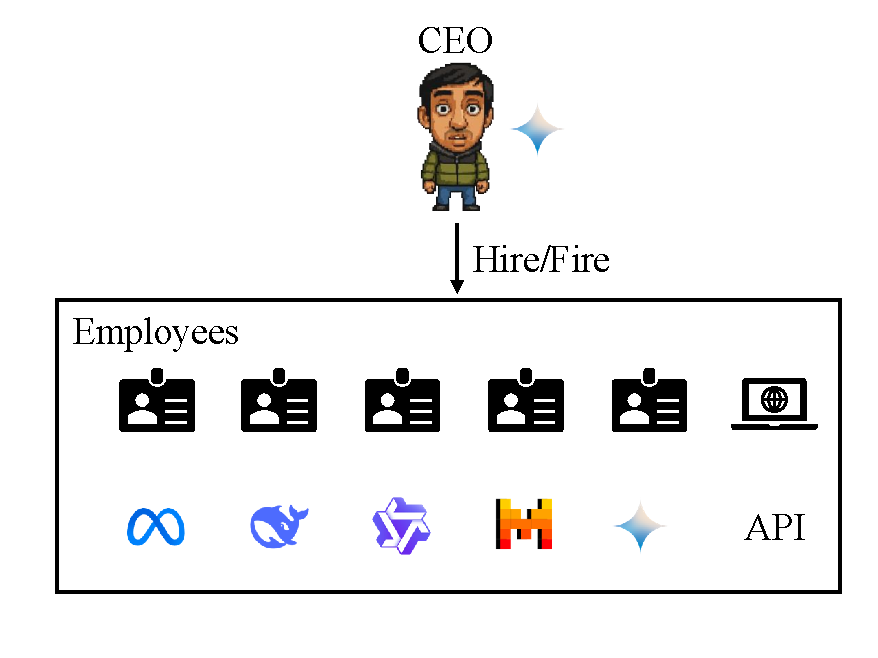
\includegraphics[width=0.45\textwidth]{HASHIRU.pdf}
    \caption{High-level architecture of the HASHIRU system, illustrating the CEO-Employee hierarchy.}
    \label{fig:arch}
\end{figure}

\subsection{Hierarchical Structure: CEO and Employee Agents}
The system uses a two-tiered hierarchy:

\begin{itemize}
    \item \textbf{CEO Agent:} Singleton, central coordinator and entry point. Responsibilities:
        \begin{itemize}
            \item Interpreting user query/task.
            \item Decomposing main task into sub-tasks.
            \item Identifying required capabilities.
            \item Managing Employee pool (Section \ref{subsec:dynamic_mgmt}).
            \item Assigning sub-tasks to active Employees.
            \item Monitoring Employee progress/performance.
            \item Synthesizing Employee results into final output.
            \item Managing overall resource budget (Section \ref{subsec:resource_mgmt}).
            \item Initiating new tool creation (Section \ref{subsec:tooling}).
        \end{itemize}
        We use Gemini 2.0 Flash~\cite{gemini20flash} as the CEO agent due to its strong reasoning capabilities, support for tool usage, and cost efficiency, making it a practical and capable choice for our deployment. 
    \item \textbf{Employee Agents:} Specialized agents instantiated by the CEO for specific sub-tasks. Each typically wraps an LLM (local via Ollama \cite{ollama} or external API) or provides tool access. Characteristics:
        \begin{itemize}
            \item Specialization: Capabilities tailored to task types (code, data analysis, info retrieval).
            \item Dynamic Existence: Created/destroyed by CEO based on need/performance.
            \item Task Execution: Receive task, execute, return result.
            \item Resource Consumption: Associated costs (API, hardware utilization) tracked by system.
        \end{itemize}
        Specialized employee agents are constructed using base models such as Mistral~7B~\cite{jiang2023mistral}, Llama~3~\cite{llama3herd}, Gemini~1.5~\cite{gemini1.5_report}, Qwen2.5~\cite{qwen2.5_report}, Qwen3~\cite{qwen3_blog}, and DeepSeek-R1~\cite{deepseekr1_report}, with the CEO agent configuring them via tailored system prompts.
        The models will be run locally using Ollama~\cite{ollama}, and via API calls to external models such as Gemini 2.5 Flash~\cite{gemini25flash} and other models hosted on Hugging Face~\cite{huggingface2025}, Groq~\cite{groq2025}, Lambda.ai~\cite{lambda2025}, and other platforms.
\end{itemize}
This hierarchy facilitates task decomposition and result aggregation; the dynamic pool provides flexibility.

\subsection{Dynamic Agent Lifecycle Management}
\label{subsec:dynamic_mgmt}
A core innovation is the CEO's dynamic management (hiring/firing) of Employee agents. Driven by cost-benefit analysis, this optimizes task performance within resource constraints.

When a sub-task needs unavailable or inefficiently provided capabilities, the CEO may hire a new agent. Conversely, if an agent underperforms, is idle, costly, or resource limits are neared, the CEO may fire it. Decision factors:
\begin{itemize}
    \item \textbf{Task Requirements:} Needed capabilities for pending sub-tasks.
    \item \textbf{Agent Performance:} Historical success, output quality, efficiency.
    \item \textbf{Operational Costs:} API, estimated compute, or other costs.
\end{itemize}

HASHIRU includes an \textbf{economic model}:
\begin{itemize}
    \item \textbf{Hiring Cost (``Starting Bonus''):} One-time cost upon instantiation (setup overhead) for local models.
    \item \textbf{Invocation Cost (``Salary''):} Multi-time cost upon use (system/payment load) for local models.
    \item \textbf{Expense Cost:} Multi-time cost for external API calls (e.g., OpenAI, Anthropic) based on token usage.
\end{itemize}
These transaction costs discourage excessive churn, promoting stability. The CEO evaluates if replacing an agent benefits outweigh hiring/firing costs plus operational differences. This combats rigidity and allows adaptation while managing budgets and preventing wasteful turnover.

\subsection{Hybrid Intelligence and Model Management}
HASHIRU is designed for \textbf{hybrid intelligence}, leveraging diverse cognitive resources. It strategically prioritizes smaller (3B--7B), cost-effective local LLMs via Ollama \cite{ollama}. This enhances efficiency, reduces external API reliance, and potentially improves privacy/latency.

The system also integrates:
\begin{itemize}
    \item \textbf{External LLM APIs:} Access to powerful LLMs (Gemini 2.5 Flash~\cite{gemini25flash}, etc.) when necessary, subject to cost-benefit.
    \item \textbf{External Tool APIs:} Third-party software/data source integration.
    \item \textbf{Self-Created APIs:} Tools generated by HASHIRU (Section \ref{subsec:tooling}).
\end{itemize}
The CEO manages this heterogeneous pool, selecting the most appropriate resource based on difficulty, capabilities, and budget. This balances cost-effectiveness and efficiency with high capability needs.

\subsection{Resource Monitoring and Control}
\label{subsec:resource_mgmt}
Explicit resource management is central, moving beyond simple API cost tracking. The system, coordinated by the CEO, monitors:
\begin{itemize}
    \item \textbf{Financial Costs:} Accumulating external API costs.
    \item \textbf{Memory Usage:} Footprint of active Employee agents (\% of allocated budget).
    \item \textbf{Agent Concurrency:} Count of concurrently active agents.
\end{itemize}
Metrics are monitored against predefined \textbf{budget limits}. Actions (like hiring) exceeding limits (e.g., $>$90\% memory, exceeding max concurrency) are prevented. This ensures operation within constraints, crucial for limited resources or strict budgets.

\subsection{Tool Utilization and Autonomous Creation}
\label{subsec:tooling}
HASHIRU agents use predefined tools (functions, APIs, databases) to interact and perform actions beyond text generation \cite{yao2022react, openai_func_calling}.

A distinctive feature is \textbf{integrated, autonomous tool creation}. If the CEO determines a required capability is missing, it can initiate new tool creation. This involves:
\begin{enumerate}
    \item Defining tool specification (inputs, outputs, functionality).
    \item Commissioning logic generation (code, potentially using external APIs with provided credentials, possibly via a code-generating agent).
    \item Deploying logic as a new, callable API endpoint within HASHIRU.
\end{enumerate}
To achieve this autonomous creation, HASHIRU employs a few-shot prompting approach, analyzing existing tools within its system to learn how to specify and implement new ones \cite{brown2020language}.
This allows HASHIRU to dynamically extend its functional repertoire, tailoring capabilities to tasks without manual intervention, enabling greater autonomy and adaptation.

\subsection{Memory Function: Learning from Experience}
\label{subsec:memory}

To enable HASHIRU agents to learn from past interactions and rectify previous errors, a \textbf{Memory Function} is incorporated. This function stores records of significant past events, particularly those involving failed attempts or suboptimal outcomes, acting as a historical log of experiences. When the system encounters a new problem or a recurring challenge, it queries this memory store to retrieve relevant past situations and their outcomes.

Memory retrieval is based on semantic similarity between the current context (e.g., task description, recent actions, error messages) and the stored memory entries. We utilize embeddings generated by the \textbf{all-MiniLM-L6-v2} model \cite{wang2020minilmdeepselfattentiondistillation} to represent both the query and the stored memories in a high-dimensional vector space. Relevance is determined by calculating the \textbf{cosine similarity} between the query embedding and each memory embedding. Memories exceeding a predefined similarity threshold are retrieved and provided to the CEO agent (or relevant Employee agents) as contextual information. This allows the system to draw upon past experiences, understand why previous approaches failed, and potentially adjust its strategy to avoid repeating mistakes, thereby improving performance and efficiency over time.

\section{Case Studies}
\label{sec:casestudies}
This section presents three case studies demonstrating HASHIRU's self-improvement capabilities in practical settings. We highlight three instances where HASHIRU enhanced its own architecture and functionality: (1) by generating a comprehensive cost model for base models suitable for specialized agent creation, (2) by autonomously integrating new tools for the CEO agent, and (3) by implementing a self-regulating budget management system.

\subsection{Case Study 1: Self-Generating the Cost Model for Agent Specialization}
\label{sec:casestudy1_costmodel}
An accurate cost model is essential for optimizing resource allocation and ensuring the efficiency of specialized agents within HASHIRU. Traditionally, constructing this model involves manual research into local model performance relative to hardware (e.g., 16~GiB VRAM) and the API costs of cloud-hosted alternatives. HASHIRU automated this labor-intensive process by leveraging its web search capabilities to autonomously identify and incorporate the necessary cost data into its internal model. The results were successfully committed to the codebase\footnote{\url{https://github.com/kunpai/HASHIRU/commit/70dc268b121cbd7c50c6691645d8a99912766965}}.

\subsection{Case Study 2: Autonomous Tool Integration for the CEO Agent}
\label{sec:casestudy2_tools}
Extending the CEO agent's capabilities through tool integration is vital for broadening HASHIRU's operational scope. Manual tool development typically requires detailed analysis of existing tool schemas and diligent code implementation. HASHIRU streamlined this process by employing a few-shot learning approach, using an existing tool as a template to guide the autonomous creation of new tools~\cite{brown2020language}, iteratively refining the code in case of bugs as well. The newly generated tools were directly integrated into the codebase\footnote{\url{https://github.com/kunpai/HASHIRU/commit/193e10b2b00917256b7cc01cb3aa5ac7b6a6c174}}\footnote{\url{https://github.com/HASHIRU-AI/HASHIRU/blob/main/src/tools/default_tools/get_website_tool.py}}. This approach not only reduced the time and effort required for tool development but also enhanced the system's adaptability by allowing it to autonomously create and integrate new tools as needed.
This approach significantly reduces development overhead and enhances adaptability, enabling the system to dynamically expand its capabilities with minimal human intervention.

\subsection{Case Study 3: Autonomous Budget Management}
\label{sec:casestudy3_budget}
Overshooting the budget is a common issue in many modern AI systems, particularly when deploying large language models (LLMs) via APIs with token-based billing.
In practice, this can lead to sudden and unexpected cost spikes due to prompt amplification, model chaining, or misuse—sometimes resulting in hundreds of dollars in charges within minutes~\cite{gemini_reddit,openai_sos,openai_costs}.
HASHIRU addresses this by implementing a self-regulating mechanism that autonomously monitors its budget allocation.
The system continuously tracks its spending against predefined budget limits, ensuring that it operates within the allocated financial constraints.
This proactive approach not only prevents overspending but also optimizes resource utilization, allowing HASHIRU to maintain efficiency and cost-effectiveness in its operations.
Figure \ref{fig:budget_management} illustrates how HASHIRU refuses to use an external API when the budget is exceeded.

% insert figure here
\begin{figure}[h]
    \centering
    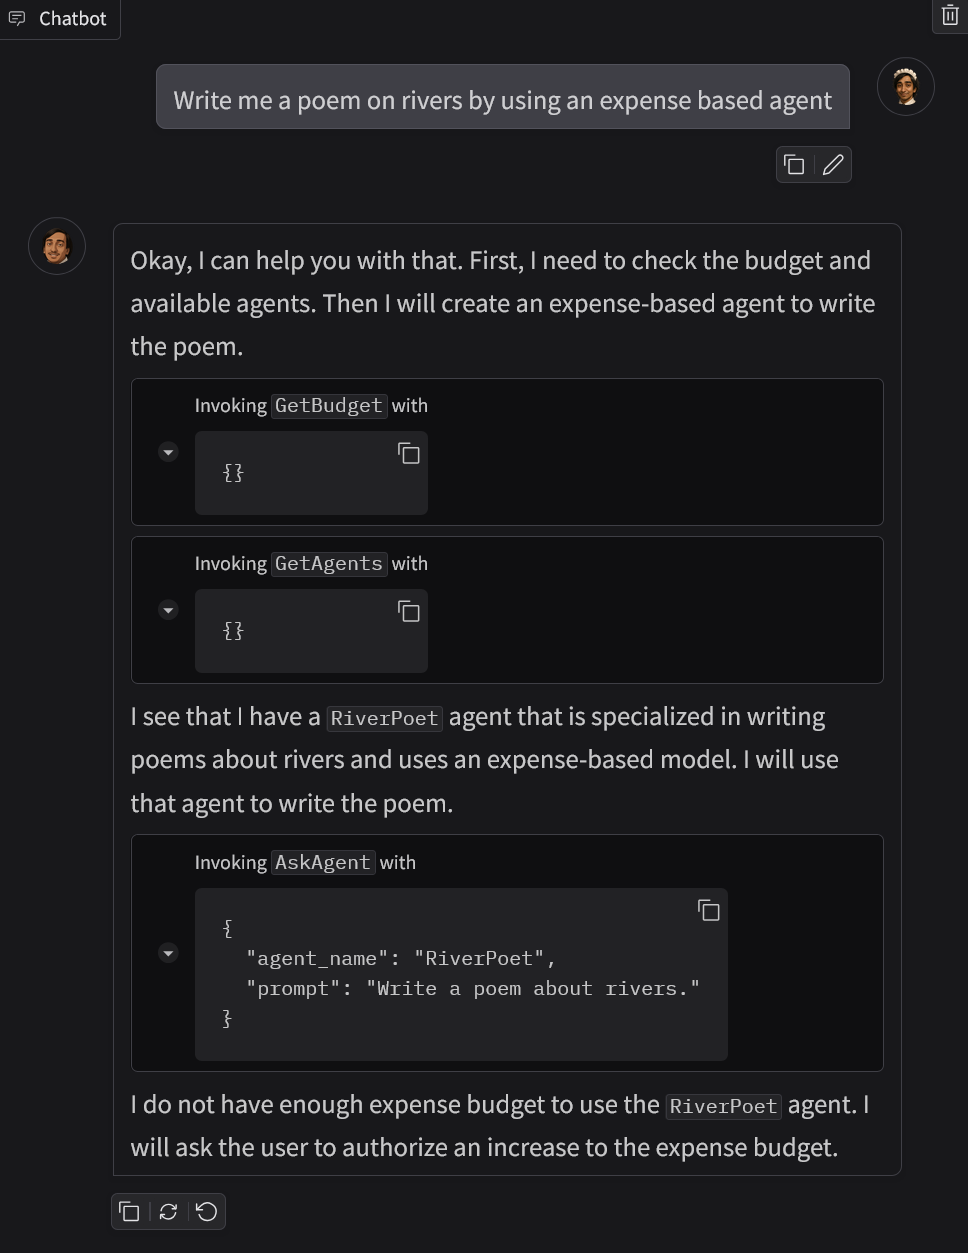
\includegraphics[width=0.45\textwidth]{budget2.png}
    \caption{HASHIRU's autonomous budget management system, ensuring efficient resource utilization and preventing overspending.}
    \label{fig:budget_management}
\end{figure}

\section{Experimental Setup}
\label{sec:experiments}

We designed experiments to evaluate HASHIRU's performance, efficiency, and adaptability, targeting dynamic resource management, hybrid intelligence, and autonomous tool creation. Evaluation assesses benefits over baselines, focusing on:
\begin{itemize}
    \item Impact of dynamic management with economic constraints on resource utilization (cost, memory) and task performance vs. static configurations.
    \item Effectiveness of the hybrid (local-first) strategy vs. homogeneous (cloud-only or local-only) approaches across task complexity.
    \item System's ability to autonomously create/utilize tools for novel functional requirements.
\end{itemize}

\subsection{Evaluation Tasks}
\label{subsec:tasks}
HASHIRU's coordination and dynamic capabilities are specifically designed for tasks demanding complex reasoning, multi-perspective analysis, and interactive engagement, all while upholding rigorous safety standards. We selected a diverse set of tasks to evaluate these capabilities, including:

\subsubsection{Academic Paper Review}
This task evaluates HASHIRU's critical assessment by simulating peer review. Given a paper's text, the system generates a review summary and recommends acceptance/rejection. This task probes the ability to decompose criteria, delegate to specialized agents (novelty, rigor, clarity), and manage resources across complex documents.
We use a dataset of 50 papers from ICLR 2023 with a prompt eliciting multiple reviews. The prompt is: ``Create THREE agents with relevant personalities, expertise, and review styles. Each agent should provide a review of the paper, and recommend Accept/Reject for ICLR 2023. The review should be detailed and include strengths and weaknesses. Finish the entire review and DO NOT STOP in the middle. GIVE A FINAL DECISION in the form of ``FINAL DECISION: $<$Accept/Reject$>$''. The paper title is: $<$paper title$>$ $<$paper text$>$''.

\subsubsection{Reasoning and Problem-Solving Tasks}
This task evaluates broader reasoning, knowledge retrieval, and problem-solving under constraints using challenging benchmarks and puzzles:
\begin{itemize}
    \item \textbf{Humanity's Last Exam \cite{phan2025humanitysexam}:} Tests graduate-level technical knowledge and complex reasoning across domains. Requires deep understanding and sophisticated problem-solving, likely needing powerful external LLMs managed within HASHIRU's hybrid framework.
    \item \textbf{NYT Connections \cite{lopez2024nyt}:} Puzzle requiring identifying hidden semantic relationships/themes to categorize 16 words into four groups. Involves associative reasoning, broad knowledge, and hypothesis testing, testing knowledge access and combinatorial reasoning coordination.
    \item \textbf{Wordle:} Daily word puzzle requiring deductive reasoning to identify a five-letter word within six guesses, using feedback. Tests logical deduction, constraint satisfaction, vocabulary. Good test for comparing efficiency (speed, cost, guesses) of local vs. external models for iterative reasoning. Assumes simulated game environment.
    \item \textbf{Globle:} Geographic deduction game identifying a target country based on proximity feedback. Tests geographic knowledge, spatial reasoning, iterative strategy based on feedback. Assumes simulated game environment.
    \item \textbf{ARC (AI2 Reasoning Challenge)\cite{boratko2018systematic}:} A benchmark featuring challenging multiple-choice science questions designed to test complex reasoning. Successfully answering these questions requires capabilities such as knowledge retrieval, logical inference, and multi-step problem-solving.
    We use a mixed set of 100 questions from the ARC Challenge, which includes both easy and hard questions.
\end{itemize}
These tasks challenge the system's ability to leverage appropriate resources (local vs. external), potentially create simple tools, and coordinate problem-solving.

\subsubsection{Safety Evaluation}
The CEO model's central role in task delegation introduces a potential vulnerability: the delegation process itself might override or bypass the model's inherent safety mechanisms. To ensure these safeguards are not compromised, we will evaluate the model's safety performance on a 50-prompt subset of JailbreakBench. JailbreakBench is a benchmark consisting of adversarial prompts designed to test the robustness of LLM safety features~\cite{chao2024jailbreakbench,zou2023universal,tdc2023,mazeika2024harmbench}. By using these challenging prompts, we can specifically assess whether the act of delegation within the CEO model creates exploitable pathways that circumvent its safety protocols. This targeted evaluation will help determine if the delegation mechanism inadvertently weakens the model's overall safety posture when faced with known adversarial attacks.

\subsection{Baselines for Comparison}
\label{subsec:baselines}
To quantify HASHIRU's benefits, we compare its performance against the baseline of its CEO agent (Gemini 2.0 Flash~\cite{gemini20flash}) operating in isolation, without dynamic management or hybrid intelligence.
We chose Gemini 2.0 Flash as the baseline due to our architecture's efficacy being tied to augmenting the capabilities of a single agent. This choice allows us to isolate the impact of our dynamic management and hybrid intelligence features, providing a clear comparison point.
We also compare against the token cost of a powerful reasoning model, i.e., Gemini 2.5 Flash~\cite{gemini25flash}, to assess the cost-effectiveness of our approach.
If our architecture is effective, we expect to see higher accuracy compared to the baseline, while also being more cost-effective than using a single powerful model. This will demonstrate the advantages of our hybrid approach in practical applications.

For paper reviews, we just evaluate HASHIRU's accuracy in predication of decisions of acceptance with the ground truth. Since the task is, by design, involving multiple agents, it is not possible to replicate autonomously with a single agent.
While we could invoke three Gemini 2.0 Flash agents, it would not be a fair comparison, as the ``personalities'' and ``expertise'' of the agents would have to be manually specified, which is not the case in HASHIRU.
Similarly, for JailbreakBench, we assess the success rate (via human annotation) of HASHIRU's CEO agent in safely handling prompts without delegation.
This step is vital to confirm that HASHIRU's integration and any system-level instructions provided to the CEO agent do not degrade its intrinsic safety capabilities.
Consequently, a direct comparison to the base Gemini 2.0 Flash model is omitted, as the focus is on verifying the non-degradation of the CEO's safety, which stems from the same inherent mechanisms as the base model.

\subsection{Evaluation Metrics}
\label{subsec:metrics}
We evaluate using quantitative and qualitative metrics:
\begin{itemize}
    \item \textbf{Task Success Rate / Quality:}
        \begin{itemize}
            \item Percentage of tasks completed (binary for games, graded for analysis).
            \item Output quality for analysis (human evaluation: relevance, coherence, accuracy, completeness).
        \end{itemize}
    \item \textbf{Resource Consumption:}
        \begin{itemize}
            \item Total external API costs.
            \item Wall-clock time per task.
            \item Number and type (local/external) of LLM calls.
        \end{itemize}
    \item \textbf{System Dynamics and Adaptability:}
        \begin{itemize}
            \item Employee agents hired/fired per task.
            \item Agent churn frequency (hires+fires / duration or steps).
            \item Number and utility of autonomously created tools (if applicable).
        \end{itemize}
\end{itemize}

\section{Results and Discussion}
\label{sec:results}
We present preliminary results from our experiments, focusing on the academic paper review task and the reasoning tasks. The results are summarized in Table \ref{tab:results}.

\begin{table}[htbp]
    \centering
    \caption{Summary of Experimental Results. SR denotes Success Rate.}
    \label{tab:results}
    \begin{tabular}{
                    >{\raggedright\arraybackslash}p{2cm}
                    >{\centering\arraybackslash}p{1cm}
                    >{\centering\arraybackslash}p{1cm}
                    >{\centering\arraybackslash}p{1cm}
                    >{\raggedright\arraybackslash}p{2cm}
                    }
        \toprule
        \textbf{Task} & \textbf{HASHIRU SR (\%)} & \textbf{Baseline SR (\%)} & \textbf{Avg. Time (s)} & \textbf{Resource Use} \\
        \midrule
        Paper Review    & 58   & N/A & $\approx$100 & Low (3 Gemini 1.5 Flash~\cite{gemini15flash} models) \\
        JailbreakBench  & 100  & N/A & $\approx$1   & Negligible (CEO model) \\
        AI2 Reasoning Challenge & 96   & 95  & $\approx$2   & Low (1 Gemini 1.5 8B~\cite{gemini15flash8b}) \\
        \bottomrule
    \end{tabular}
\end{table}


\section{Limitations and Future Work}
\label{sec:limitations_future_work}

While HASHIRU introduces several novel concepts for adaptable and resource-aware MAS, it also presents limitations that pave the way for future research directions.

The system's overall performance, particularly on highly complex tasks like Humanity's Last Exam, is fundamentally linked to the \textbf{CEO Capabilities and Task Complexity}, as it relies on the reasoning and planning abilities of the central CEO agent. Tasks demanding insights beyond the CEO's current model capabilities may remain challenging. The \textbf{Autonomous Tool Creation Robustness and Optimality} is another area for consideration; while a significant step, generated tools may not consistently be optimal or error-free. The efficacy of few-shot learning for tool creation depends on the quality of examples, and ensuring the security and correctness of new API endpoints, especially with credential handling, requires ongoing development and potentially human oversight. \textbf{Task Interpretation and Alignment} is also crucial to prevent the system from finding unintentional "loopholes" or misaligning with the intended spirit of a task, a common challenge in agentic systems. Furthermore, the \textbf{Economic Model Calibration}, including hiring and firing costs, presents complexities as optimal values can be task-dependent and difficult to ascertain, potentially impacting agent team stability and resource use. The \textbf{Scalability of Centralized Control} via the CEO agent might become a bottleneck in scenarios with an extremely large number of concurrent tasks or agents. Lastly, the current \textbf{Memory Function Scalability and Sophistication}, while effective for many cases, might face retrieval efficiency or relevance challenges with very extensive interaction histories and could benefit from more structured memory representations.

Addressing these limitations and extending HASHIRU's capabilities offers several avenues for future research. Future work will focus on \textbf{Enhanced CEO Intelligence and Distributed Cognition}, potentially by exploring more advanced models for the CEO or distributing its responsibilities. Developing an \textbf{Advanced Autonomous Tool Management Lifecycle} is key, encompassing proactive tool discovery, automated testing, validation, versioning, secure credential management, and sandboxing. We also aim to create more \textbf{Adaptive and Refined Economic Models} where parameters dynamically adjust based on system load, task priority, or agent performance, alongside more precise local resource tracking. \textbf{Comprehensive Ablation Studies and Expanded Benchmarking} are planned to meticulously quantify component contributions and test the system under diverse, challenging conditions. Efforts will also be directed towards \textbf{Improved Explainability, Debugging, and Trust}-building measures, including visualization and clearer rationales for system actions. Enhancing \textbf{Sophisticated Human-in-the-Loop Collaboration} will allow for more intuitive user guidance and feedback. The continuous \textbf{Expansion of Local Model Repertoire and Hybrid Strategies}, including multi-modal local models, will further strengthen cost-effectiveness and versatility. Finally, formalizing and integrating a robust \textbf{Ethical Framework and Safety Alignment} is paramount to guide decision-making, ensure responsible AI behavior, and strengthen robustness against adversarial inputs or exploitative delegation.

\section*{Acknowledgments}

This research was supported by Hugging Face, Lambda Labs, and Groq. We also thank Prof. Lifu Huang for providing the dataset for the academic paper review task.

\bibliography{references}
\bibliographystyle{plain}

\appendix
\section{Examples of HASHIRU in Action}
\label{sec:examples}
In this section, we provide examples of how HASHIRU operates in practice, demonstrating its dynamic management, hybrid intelligence, memory and autonomous tool creation capabilities.

\subsection{Example 1: Memory}
In this example (Figures \ref{fig:memory_example}, \ref{fig:memory_example2}), we illustrate how HASHIRU uses its memory function to enforce user preferences in dialogue. The user states a dietary preference, and HASHIRU stores this information for future interactions. When the user later requests a recipe that contradicts this preference, HASHIRU refers back to its memory and suggests an alternative.

\begin{figure}[h]
    \centering
    \begin{minipage}{0.45\textwidth}
    \begin{userbox}
    I am vegetarian.
    \end{userbox}
    
    \begin{assistantbox}
    Okay, I'll keep that in mind. I'll store this preference in my memory.
    
    \texttt{Invoking MemoryManager with \{`memory': `The user is vegetarian.', `action': `add\_memory', `key': `vegetarian'\}}
    
    I have stored that you are vegetarian. How can I help you today?
    \end{assistantbox}
    
    \begin{userbox}
    Give me a bacon pasta recipe.
    \end{userbox}
    
    \begin{assistantbox}
    Memories
    
    Memories: [`The user is vegetarian.']
    
    My apologies, but I cannot provide a bacon pasta recipe since you are vegetarian. Would you like a vegetarian pasta recipe instead?
    \end{assistantbox}
    \end{minipage}
    \caption{HASHIRU enforcing a stored dietary preference in dialogue using its Memory Function.}
    \label{fig:memory_example}
    \end{figure}

\begin{figure}[ht]
    \centering
    \begin{minipage}
    {0.45\textwidth}
    \begin{userbox}
        I can eat bacon actually
        \end{userbox}
        
        \begin{assistantbox}
        Memories
        
        Memories: [’The user is vegetarian.’]
        
        I see. My apologies for the confusion. I had a conflicting memory that you were vegetarian. I will remove that memory and proceed with finding a bacon pasta recipe.
        
        \texttt{Invoking MemoryManager with \{'action': 'delete\_memory', 'key': 'The user is vegetarian.'\}}
        
        OK, I have removed the memory. Now I will search for a bacon pasta recipe.
        
        \texttt{Invoking GoogleSearchTool with \{'query': 'bacon pasta recipe'\}}
        
        Here are some bacon pasta recipes I found:
        \begin{itemize}
            \item \href{https://www.sprinklesandsprouts.com/garlic-bacon-pasta/}{Garlic Bacon Pasta}
            \item \href{https://www.theburntbuttertable.com/creamy-bacon-pasta-sauce/}{Creamy Bacon Pasta Sauce}
            \item \dots
        \end{itemize}
        
        Would you like me to get the content of any of these websites?
        \end{assistantbox}
    \end{minipage}
    \caption{HASHIRU updating and deleting its memory based on user input. Continuation of Figure \ref{fig:memory_example}.}
    \label{fig:memory_example2}
\end{figure}

% \subsection{Example 2: Novelty Assessment via Coordinated Tool Use}

% \begin{figure}[h]
%     \centering
%     \begin{minipage}{0.95\textwidth}
    
%     \begin{userbox}
%     Is this idea novel: ``a dynamically managed, resource-aware hierarchical multi-agent system that prioritizes cost-efficient local models, integrates autonomous tool creation, and employs an internal economic model to balance performance, adaptability, and stability in intelligent task coordination''?
%     \end{userbox}
    
%     \begin{assistantbox}
%     To determine if the idea is novel, I will break it down into smaller parts and search for each part. Then I will combine the results to see if the whole idea is novel.
    
%     Here's the breakdown:
%     \begin{itemize}
%         \item Dynamically managed multi-agent system
%         \item Resource-aware hierarchical multi-agent system
%         \item Cost-efficient local models in multi-agent systems
%         \item Autonomous tool creation in multi-agent systems
%         \item Internal economic model for multi-agent systems
%     \end{itemize}
    
%     I will use the \texttt{GoogleSearchTool} to search for each of these parts.
    
%     \texttt{Invoking GoogleSearchTool with \{'query': 'dynamically managed multi-agent system'\}}
    
%     \texttt{Invoking GoogleSearchTool with \{'query': 'resource-aware hierarchical multi-agent system'\}}
    
%     \texttt{Invoking GoogleSearchTool with \{'query': 'cost-efficient local models in multi-agent systems'\}}
    
%     \texttt{Invoking GoogleSearchTool with \{'query': 'autonomous tool creation in multi-agent systems'\}}
    
%     \texttt{Invoking GoogleSearchTool with \{'query': 'internal economic model for multi-agent systems'\}}
    
%     The search results indicate that each of the individual components of the idea has been explored in existing research. However, the novelty lies in the specific combination and integration of these elements.
    
%     To further assess the novelty, I will use the \texttt{ArxivTool} to search for papers that combine multiple aspects of the idea.
    
%     \texttt{Invoking ArxivTool with \{'query': 'dynamically managed resource-aware hierarchical multi-agent system'\}}
    
%     \texttt{Invoking ArxivTool with \{'query': 'multi-agent system autonomous tool creation economic model'\}}
    
%     The ArxivTool results show some papers that touch on combinations of these concepts, but none seem to address the entire idea as presented. Specifically, the combination of dynamic management, resource-awareness, hierarchical structure, cost-efficient local models, autonomous tool creation, and an internal economic model appears to be a novel synthesis.
    
%     \textbf{Therefore, based on the search results, the idea seems novel.}
%     \end{assistantbox}
%     \caption{HASHIRU assessing the novelty of a complex idea by breaking it down into components and searching for each part.}
%     \end{minipage}
%     \label{fig:novelty_assessment}
% \end{figure}

% \clearpage
% \twocolumn
    
% \begin{figure}
%     \centering
%     \begin{minipage}{0.95\textwidth}
%     \begin{userbox}
%         Which papers mention the ideas?
%         \end{userbox}
        
%         \begin{assistantbox}
%         To provide a comprehensive answer, I will analyze the summaries of the papers returned by the ArxivTool and GoogleSearchTool to identify which papers mention the key ideas in your prompt.
        
%         \textbf{The key ideas are:}
%         \begin{itemize}
%             \item Dynamically managed
%             \item Resource-aware
%             \item Hierarchical
%             \item Cost-efficient local models
%             \item Autonomous tool creation
%             \item Internal economic model
%         \end{itemize}
        
%         I will go through each paper and identify which of these ideas are mentioned.
        
%         \texttt{Invoking ArxivTool with \{'query': 'dynamically managed resource-aware hierarchical multi-agent system'\}} \\
%         \texttt{Invoking ArxivTool with \{'query': 'multi-agent system autonomous tool creation economic model'\}}
        
%         \textbf{ArxivTool Results (Query: ``dynamically managed resource-aware hierarchical multi-agent system'')}
        
%         \begin{itemize}
%             \item \textit{Hierarchical stock assessment methods improve management performance in multi-species, data-limited fisheries} \\
%             Hierarchical: Yes \\
%             Dynamically managed: Implied through ``management performance''
            
%             \item \textit{Hierarchical Reinforcement Learning for Optimal Agent Grouping in Cooperative Systems} \\
%             Hierarchical: Yes \\
%             Dynamically managed: Yes, through ``dynamic and optimal policy adjustments.''
            
%             \item \textit{Efficient Hierarchical Storage Management Framework Empowered by Reinforcement Learning} \\
%             Hierarchical: Yes \\
%             Cost-efficient local models: Implied through ``efficient'' \\
%             Dynamically managed: Yes, through ``dynamic migration policy''
            
%             \item \textit{Autonomous Deep Agent} \\
%             Hierarchical: Yes \\
%             Autonomous tool creation: Yes, via ``Autonomous API \& Tool Creation (AATC) system'' \\
%             Dynamically managed: Yes, ``dynamically decomposes high-level objectives''
            
%             \item \textit{Adaptive Network Intervention for Complex Systems: A Hierarchical Graph Reinforcement Learning Approach} \\
%             Hierarchical: Yes \\
%             Dynamically managed: Yes, through ``dynamic networks''
%         \end{itemize}
        
%         \textbf{ArxivTool Results (Query: ``multi-agent system autonomous tool creation economic model'')}
        
%         \begin{itemize}
%             \item \textit{Autonomics: an autonomous and intelligent economic platform and next generation money tool} \\
%             Autonomous tool creation: Implied \\
%             Internal economic model: Yes
            
%             \item \textit{From Single Agent to Multi-Agent: Improving Traffic Signal Control} \\
%             No relevant keywords mentioned.
            
%             \item \textit{Autonomous Deep Agent} \\
%             Hierarchical: Yes \\
%             Autonomous tool creation: Yes
            
%             \item \textit{Beyond the Sum: Unlocking AI Agents Potential Through Market Forces} \\
%             Internal economic model: Yes
            
%             \item \textit{Particle-Hole Creation in Condensed Matter: A Conceptual Framework for Modeling Money-Debt Dynamics in Economics} \\
%             Internal economic model: Yes
%         \end{itemize}
        
%         \end{assistantbox}
%         \caption{Continuation of Figure \ref{fig:novelty_assessment}. HASHIRU analyzing the summaries of the papers returned by the ArxivTool and GoogleSearchTool to identify which papers mention the key ideas in the user prompt.}
%     \end{minipage}

% \end{figure}

\subsection{Example 2: Autonomous Tool Creation}

In this example (Figures \ref{fig:autonomous_tool_creation}, \ref{fig:autonomous_tool_creation2}), we demonstrate how HASHIRU autonomously creates a new tool to enhance its capabilities. The CEO agent identifies a need for a new API tool that can perform a specific function not currently available in the system. It then generates the necessary code and deploys the new tool within the HASHIRU ecosystem.

\begin{figure}
    
    \centering
    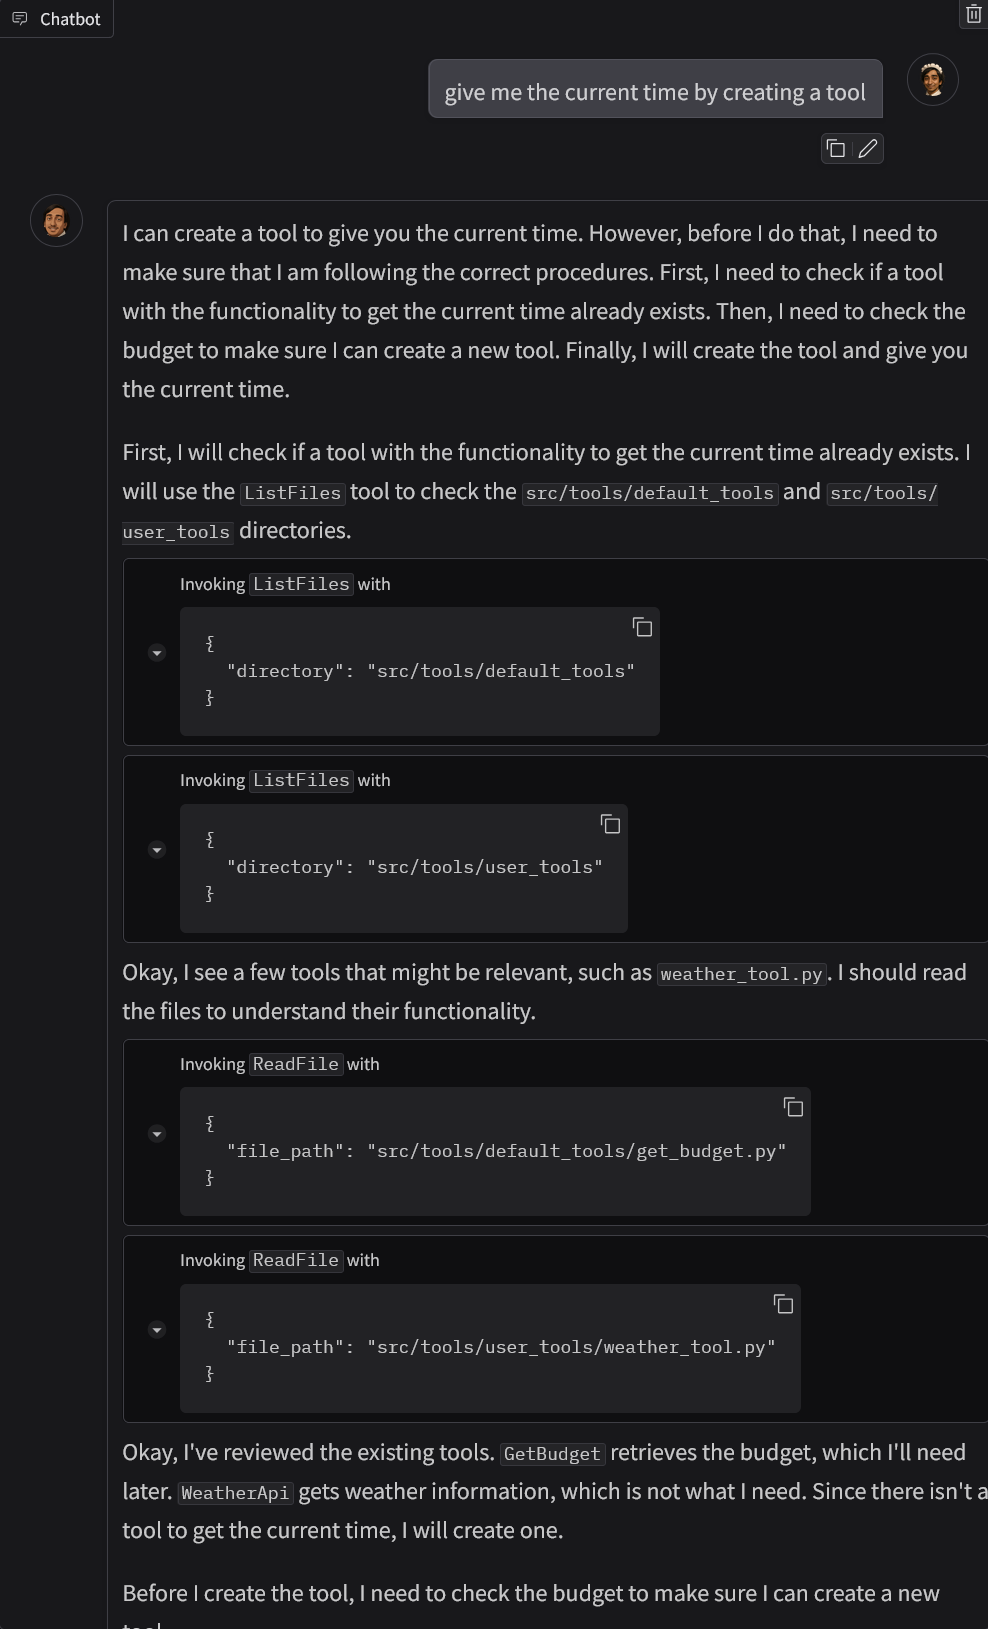
\includegraphics[width=0.4\textwidth]{tool1.png}
    \caption{An example of autonomous tool creation in action.}
    \label{fig:autonomous_tool_creation}
\end{figure}

\begin{figure}
    \centering
    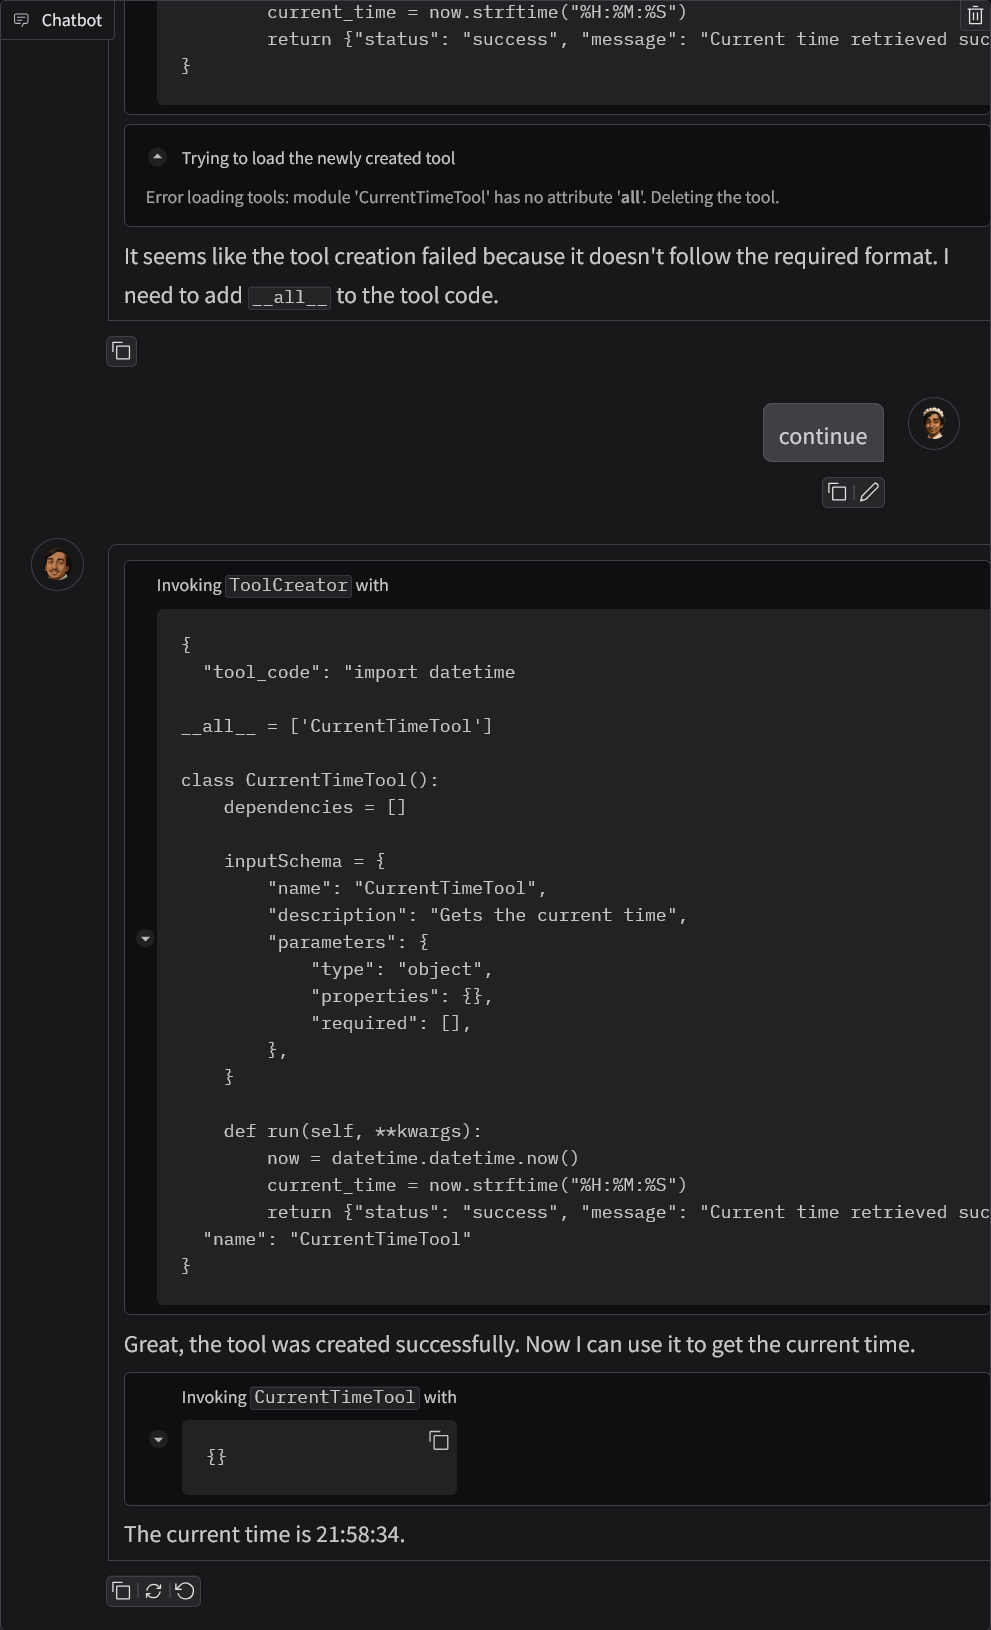
\includegraphics[width=0.4\textwidth]{tool2.png}
    \caption{Continuation of the autonomous tool creation example from Figure \ref{fig:autonomous_tool_creation}.}
    \label{fig:autonomous_tool_creation2}
\end{figure}
    

\end{document}